\documentclass[12pt]{article}

\usepackage{amsmath, amssymb, amsthm, graphicx, mathtools}
\usepackage{indentfirst}
\usepackage{tikz}
\usepackage[colorlinks=true]{hyperref}

\title{SAT Solvers for Sudoku Problems}

\author{
  Huber, Gregory \\
  V00862879
  \and
  Hsu, Leo \\
  V00928098
  \and
  Kashike Umemura \\
  V00909836
}

\usepackage[left=1in, right=1in, top=1in, bottom=1in]{geometry}

%commands for the various number spaces
\newcommand{\N}{\mathbb{N}}
\newcommand{\Z}{\mathbb{Z}}
\newcommand{\Q}{\mathbb{Q}}
\newcommand{\R}{\mathbb{R}}
\newcommand{\C}{\mathbb{C}}
\newcommand{\T}{\mathbb{T}}
\newcommand{\K}{\mathbb{K}}
\newcommand{\Zn}{\mathbb{Z}_{n}}
\newcommand{\F}{\mathbb{F}}

%commands for the different braces
\newcommand{\pa}[1]{\left(#1\right)}
\newcommand{\bra}[1]{\left[#1\right]}
\newcommand{\cur}[1]{\left\{#1\right\}}

\DeclarePairedDelimiter\abs{\lvert}{\rvert}

\graphicspath{{./images/}}
% \includegraphics[scale=0.5]{image_name_in_folder.png}

\usepackage{listings, color}

\definecolor{dkgreen}{rgb}{0,0.6,0}
\definecolor{gray}{rgb}{0.5,0.5,0.5}
\definecolor{mauve}{rgb}{0.58,0,0.82}

\lstset{frame=tb,
  language=SQL,
  aboveskip=3mm,
  belowskip=3mm,
  showstringspaces=false,
  columns=flexible,
  basicstyle={\small\ttfamily},
  numbers=none,
  numberstyle=\tiny\color{gray},
  keywordstyle=\color{blue},
  commentstyle=\color{dkgreen},
  stringstyle=\color{mauve},
  breaklines=true,
  breakatwhitespace=true,
  tabsize=4
}

\begin{document}

\maketitle

\section{Introduction and Background}

\indent In this project, programs are written to fully solve partially solved Sudoku puzzles using the SAT solver, \texttt{miniSAT}. In particular, we have programs \texttt{sud2sat1} and \texttt{sat2sud1} that, respectively, reads a single Sudoku puzzle before converting it to a CNF formula which is then suited to be inputted to \texttt{miniSAT} to be solved, and translates the output produced by \texttt{miniSAT} for a given puzzle instance back to a solved Sudoku puzzle.
\newline

The general approach in which \texttt{sud2sat1} is implemented is that for each cell $(i, j)$ in the puzzle taking on a possible value $k$ we have a propositional variable $x_{ijk}$, and for each of $x_{ijk}$ we create a unique integer for it given by
\begin{equation}\label{base9}
81 \times (i-1) + 9 \times (j-1) + (k-1) + 1
\end{equation}
where we associate $ijk$ with a base-9 number with the final additional $1$ for the encoding to be suited for $\texttt{miniSAT}$. With this encoding for the propositional variables, we start with a formula with the `minimal' encoding for the constraints (page 5 of the CSC 322 lecture slides on SAT Solvers). Finally, we add to the formula singular terms (conjuncts with only one variable) for each known value from the given puzzle before we feed the formula (in DIMACS format) to \texttt{miniSAT}.
\newline

For \texttt{sat2sud1}, the approach is fairly straightforward. That is, we parse through the output of \texttt{miniSAT} (a satisfying assignment) to look for all the positive integer values (that correspond to the propositional variables that are assigned \texttt{TRUE}) and, in essence, recover the triple $(i, j, k)$ from equation (\ref{base9}) and reconstruct the puzzle with cell $(i, j)$ taking on value $k$.
\newline

The extended tasks are also done in this project, where we have programs \texttt{sud2sat2} (\emph{efficient encoding}), \texttt{sud2sat2}, \texttt{sat2sud3} (\emph{extended encoding}), and \texttt{sat2sud3}. Note that since for each $1 \leq i \leq 3$, \texttt{sat2sud}$i$ simply translates a truth assignment of the propositional variables back to a solved puzzle configuration, it makes sense that their implementations coincide with one another, and it turns out to be the case for us this project. Moreover, we also observe that \texttt{sud2sat2} is obtained from \texttt{sud2sat1} by adding an additional constraint, and that \texttt{sud2sat3} is obtained from \texttt{sud2sat2} by adding 3 additional constraints.

\section{Performance Evaluation}

The statistics of every task were saved to a text file and analysed. The specific attributes that are analysed are \texttt{Number of clauses}, \texttt{Memory usage}, and \texttt{CPU time}.

\begin{figure}[hbt!]
	\centering
	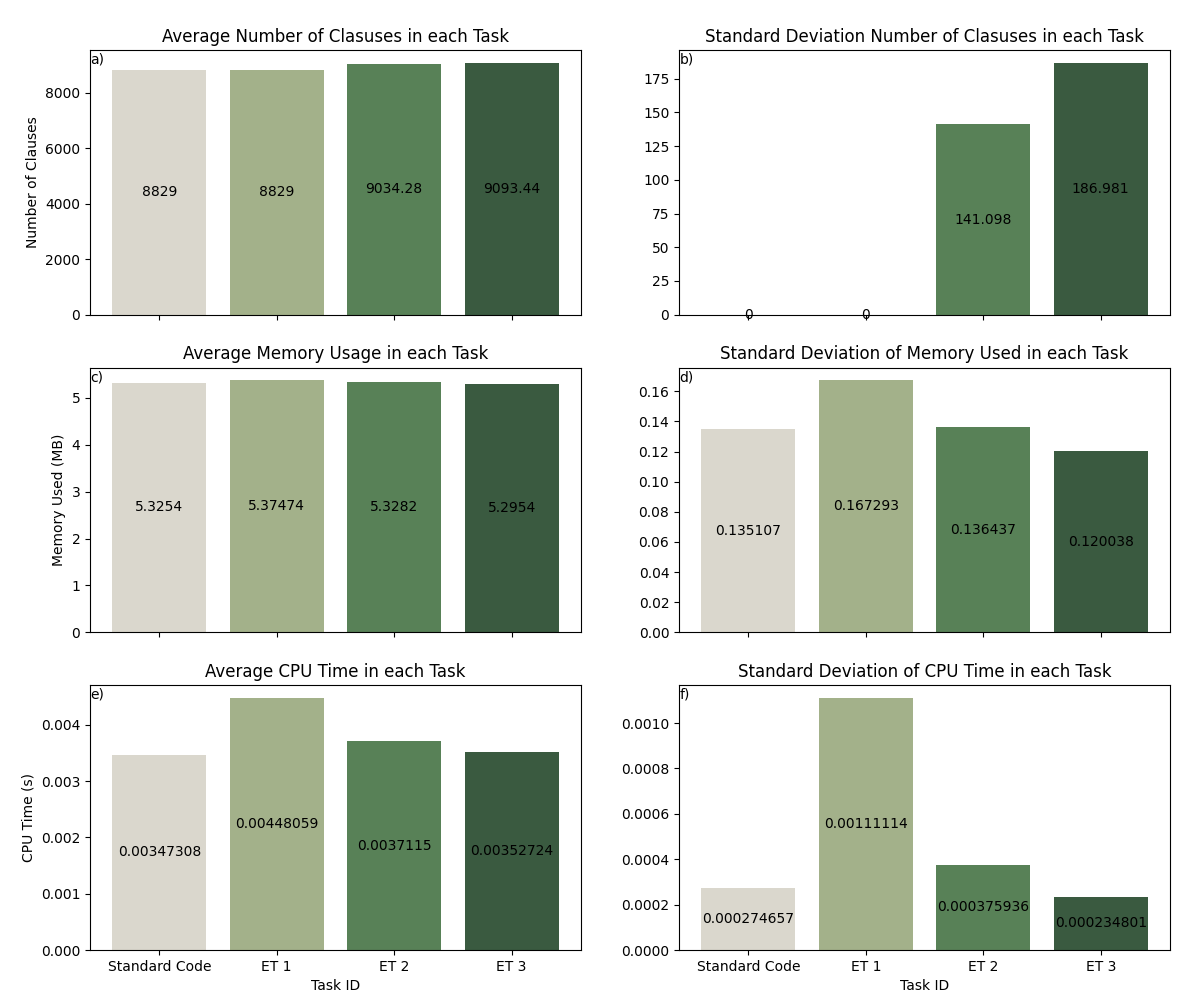
\includegraphics[scale=0.5]{average_std}
	\caption{Average of the attributes \texttt{Number of Clauses}, \texttt{Memory Usage}, and \texttt{CPU Time} are shown on the charts a), c), and e) and the standard deviations of these attributes are shown on the charts b), d), and f) for each of the tasks which are labelled on the x-axis at the bottom of the figure. Standard Code is the original objective of this project, ET 1 represents the extended task 1, ET 2 the extended task 2, and ET 3 the extended task 3. }
\end{figure}

\textit{Figure 1} shows the averages and the standard deviation of each aforementioned attributes. In terms of averages, the \texttt{Number of clauses} and \texttt{Memory usage} the differences were insignificant for the two attributes. But for the \texttt{CPU time}, the extended task 2 took longer than any other task. This indicates that having more clauses does not necessary mean that it will take a longer \texttt{CPU time}. On the other hand, if we look at the standard deviations, for \texttt{Number of clauses}, there the minimum encoding and the extended task 1 has 0 as the standard deviation. This is because the standard code and the extended task 1 use the \textit{minimal encoding}, so these encodings use the least number of clauses. However, extended task 2 and 3 have some variance which are approximately 141 and 187 respectively. The standard deviation of \texttt{Memory used} were similar for the standard code, extended task 2 and extended task 3. Extended task 1 had a standard deviation value of approximately 0.03MB greater than the other values. As for the last attribute, \texttt{CPU time} the extended task 1 has the largest standard deviation, this would be expected, as the difference in the difficulty of the hard Sudokus are not likely to be similar, where ones with less pre-filled in cells are significantly harder.

\begin{figure}[hbt!]
	\centering
	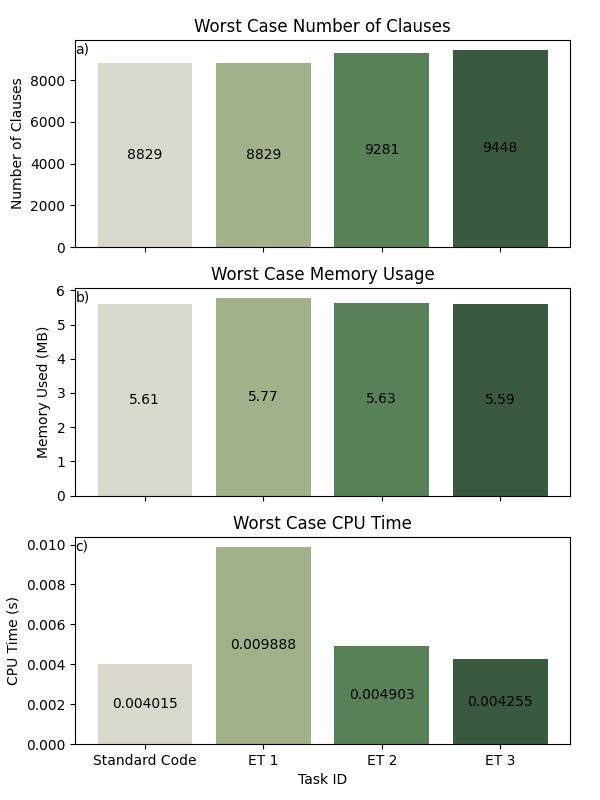
\includegraphics[scale=0.5]{worst_case}
	\caption{Attributes (\texttt{Number of clauses}, \texttt{Memory usage}, and \texttt{CPU time}) for each task in their worst results that were recorded by \texttt{minisat}. Just like \textit{Figure 1} the tasks are labelled on the x-axis. a) represents the worst case number of clauses for each task, b) represents the worst case memory usage for each task and similarly c) shows the worst case CPU time for each task.}
\end{figure}

\textit{Figure 2} shows the worst case values of attributes \texttt{Number of clauses}, \texttt{Memory usage}, and \texttt{CPU time}. The task that has the most clauses is extended task 3. This is expected since this encoding is called the \textit{extended encoding}, which uses all 4 of the additional constraints. The task with the second most clauses is the extended task 2, which includes the first additional constraints. The \textit{minimal encoding} and the extended task 1 have the same number of clauses because they both use the same constraints, which is minimal. The \texttt{Memory usage} of all tasks were similar for the worst case. But on the other hand, the \texttt{CPU time} is significantly worse for extended task 1. This supports the possibility that having more clauses does not increase computation time but having a difficult Sudoku puzzle does increase it.

\end{document}
